		From \eqref{prop:lin-eq-unit-mat},
\begin{align}
	\myvec{ -1 & 1\\  2 & -4 }\vec{n} = \myvec{1 \\ 1 }
	\\
	\implies 
	\augvec{2}{1}{ 
	-1 & 1 & 1
	\\  
	2 & -4 & 1
	}
     \xleftrightarrow[]{R_2 \leftarrow R_2+2R_1}
	\augvec{2}{1}{ 
	-1 & 1 & 1
	\\ 
	0 & -2 & 3 
	}
	\\
     \xleftrightarrow[]{R_1 \leftarrow 2R_1+R_2}
	\augvec{2}{1}{ 
	-2 & 0 &5 
	\\ 
	0 & -2 & 3 
	}
	\implies \vec{n} = -\frac{1}{2}\myvec{ 5 \\ 3}
\end{align}
Thus, from
		\eqref{prop:lin-eq-unit},
the equation of the line is
\begin{align}
 \myvec{ 5 & 3}\vec{x}  &= -2
\end{align}
See 
   \figref{fig:chapters/11/10/2/7/Line_AB}.
\begin{figure}[H]
  \centering
   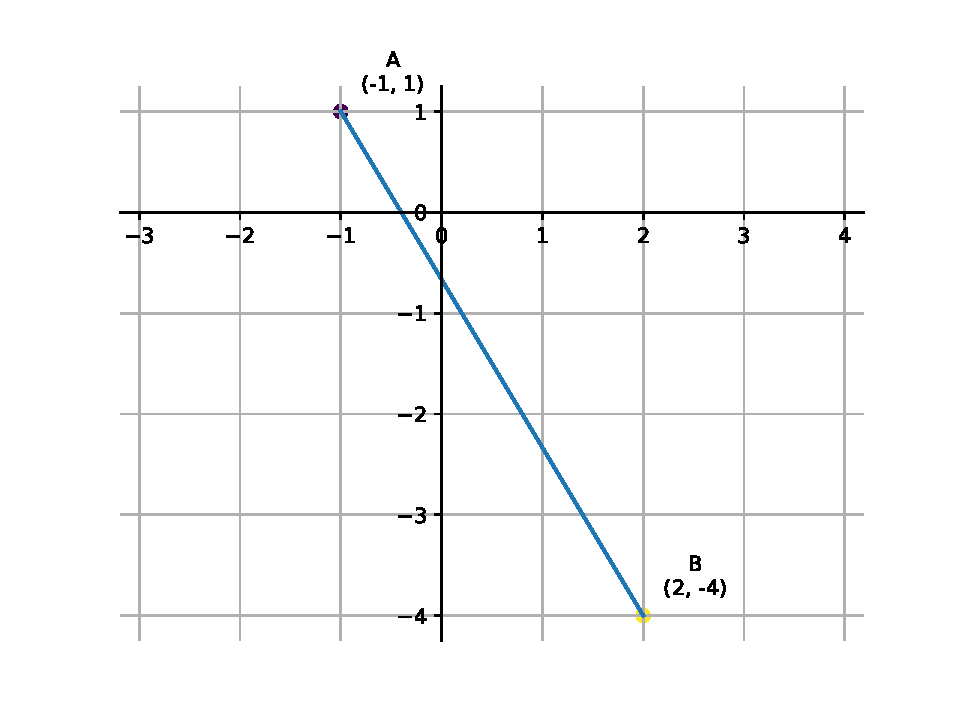
\includegraphics[width=0.75\columnwidth]{chapters/11/10/2/7/figs/fig.pdf}
   \caption{}
   \label{fig:chapters/11/10/2/7/Line_AB}
\end{figure}




